\subsection{Monotonicity formula}

If we instead integrated the stress-energy tensor over the light cone, we can obtain a monotonicity formula for the energy when restricted to slices of the light cone in time. Before we state the formula, we will need to introduce some notation. We denote the forward light cone by 
	\[ C := \{(t,x ) \in \R^{1 + 2} : r \leq t\} \]
and its restrictions to some time interval $I \subseteq [0, \infty)$ as well as time-slices by 
	\begin{align*}
		C_I 
			&:= C \cap (I \times \R^2), \\
		S_{t}
			&:= C \cap (\{t\} \times \R^2).
	\end{align*}
The \emph{null boundary} $\partial C_I$ denotes the boundary of the time-slab $C_I$ modulo the top and bottom time-slices. Due to singularities on the null boundary, we will also consider the shifted light cone 
	\[ C^\delta := (\delta, 0) + C. \]
Accordingly, we have 
	\begin{align*}
		C^\delta_I
			&:= C_I \cap C^\delta, \\
		S^\delta_t
			&:= S_t \cap C^\delta,		
	\end{align*}	
In view of the null boundary, we define the null frame $\{L, \underline L, \slashed\partial\}$ to be the vector fields given by 
	\begin{align*}
		L
			&:= \partial_t + \partial_r, \\
		\underline L
			&:= \partial_t - \partial_r,\\
		\slashed \partial
			&:= \frac1r \partial_\theta . 		
	\end{align*}
	
	
	\begin{figure}[h]
		\begin{center}
			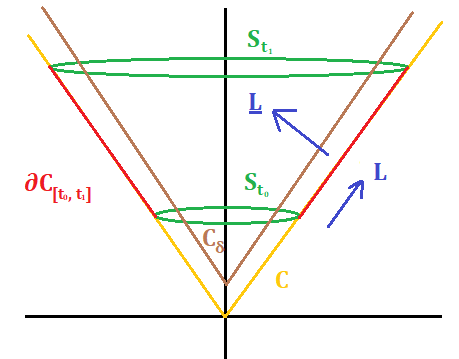
\includegraphics{graphics/cone}
			\caption{The light cone $C$, its vertical shift $C^\delta$, the time-slices $S_{t}$, the null boundary $\partial C_{[t_0, t_1]}$, and the null frame $\{L, \underline L, \slashed\partial\}$. }
		\end{center}	
	\end{figure}	
Contracting the stress-energy tensor $T_{\alpha \beta}$ with the vector field $\partial_t$ and then integrating then over the slab of the light cone $C_{[t_0, t_1]}$, we obtain in view of the divergence-free property and Stokes' theorem the  \emph{monotonicity formula}
	\begin{equation}
		\cE_{S_{t_1}} [\phi] = \cF_{[t_0, t_1]} [\phi] + \cE_{S_{t_0}} [\phi],
		\label{eq:mono}
		\tag{$\uparrow$}
	\end{equation}	
where $\cE_{S_{t_0}} [\phi]$ denotes the energy on the time-slice $S_{t_0}$, 
	\[ \cE_{S_{t_0}} [\phi] := \int_{S_{t_0}} |\partial_t \phi|^2 + |\nabla_x \phi|^2 \, dx ,\]
and $\cF_{[t_0, t_1]} [\phi]$ denotes the \emph{flux} of the wave map on the null-boundary of the light cone,
	\[
		\cF_{[t_0, t_1]} [\phi] := \int_{\partial C_{[t_0, t_1]}} \left( \frac14 |L \phi|^2 + \frac12 |r^{-1} \partial_\theta \phi|^2 \right) \, dA.
	\]
The key observation is that the flux is non-negative, hence \eqref{mono} is indeed a monotonicity formula for the energy on time-slices of the light cone $\cE_{S_t} [\phi] \nearrow$. 
	